% ROW 1: Phần đầu trang & Hình 6
\noindent
\begin{minipage}[t]{0.25\textwidth}
  \vspace{0pt}%
  \centering
  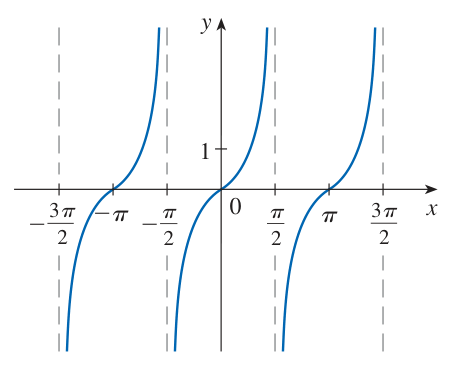
\includegraphics[width=\linewidth]{images/p0155_fig1.png}
  
  \vspace{4pt}
  \raggedright
  {\small\noindent\textbf{\textsf{HÌNH 6}}\par
  \vspace{1pt}
  \noindent $y = \tan x$\par}
\end{minipage}%
\hfill
\begin{minipage}[t]{0.71\textwidth}
  \vspace{0pt}%
  \noindent của $\pi/2$, do đó $y = \tan x$ có các điểm gián đoạn vô hạn khi $x = \pm\pi/2, \pm 3\pi/2, \pm 5\pi/2$, và cứ tiếp tục như vậy (xem Hình 6).

  \vspace{6pt}
  Hàm ngược của mọi hàm số liên tục và đơn ánh cũng là một hàm liên tục. (Kết quả này được chứng minh trong Phụ lục F, nhưng trực giác hình học khiến điều đó có vẻ hợp lý: đồ thị của $f^{-1}$ nhận được bằng cách lấy đối xứng đồ thị của $f$ qua đường thẳng $y = x$. Vì vậy, nếu đồ thị của $f$ không bị đứt đoạn thì đồ thị của $f^{-1}$ cũng vậy.) Do đó, các hàm lượng giác ngược là liên tục.

  \vspace{6pt}
  Trong Mục 1.4, chúng ta đã định nghĩa hàm mũ $y = b^x$ sao cho lấp đầy các khoảng trống trên đồ thị của $y = b^x$ tại những điểm $x$ hữu tỉ. Nói cách khác, chính định nghĩa của $y = b^x$ làm cho nó trở thành một hàm liên tục trên $\mathbb{R}$. Do đó, hàm ngược của nó $y = \log_b x$ liên tục trên $(0, \infty)$.
\end{minipage}

\vspace{10pt}

% ROW 2: Định lý 7 & Ghi chú lề Mục 1.5
\noindent
\begin{minipage}[t]{0.25\textwidth}
  \vspace{0pt}%
  {\footnotesize\noindent Các hàm lượng giác ngược được ôn lại trong Mục 1.5.\par}
\end{minipage}%
\hfill
\begin{minipage}[t]{0.71\textwidth}
  \vspace{0pt}%
  \begin{definitionbox}
  \noindent\thmnum{7}\;\; \textbf{\textsf{\color{stewartred}Định lý}}\quad Các loại hàm số sau đây liên tục tại mọi số thuộc tập xác định của chúng:
  \vspace{6pt}
  \begin{center}
  \small\renewcommand{\arraystretch}{1.25}
  \begin{tabular}{@{}l@{\hspace{18pt}}l@{\hspace{18pt}}l@{}}
  \textcolor{stewartred}{\textbullet}\; hàm đa thức & \textcolor{stewartred}{\textbullet}\; hàm phân thức hữu tỉ & \textcolor{stewartred}{\textbullet}\; hàm căn thức \\
  \textcolor{stewartred}{\textbullet}\; hàm lượng giác & \textcolor{stewartred}{\textbullet}\; hàm lượng giác ngược & \\
  \textcolor{stewartred}{\textbullet}\; hàm mũ & \textcolor{stewartred}{\textbullet}\; hàm logarit &
  \end{tabular}
  \end{center}
  \end{definitionbox}
\end{minipage}

\vspace{10pt}

% ROW 3: Ví dụ 6 & 7 + đoạn chuyển tiếp
\noindent
\begin{minipage}[t]{0.25\textwidth}
  \mbox{}
\end{minipage}%
\hfill
\begin{minipage}[t]{0.71\textwidth}
  \vspace{0pt}%
  \noindent\textbf{\textsf{\color{stewartcyan}VÍ DỤ 6}}\quad Hàm số $f(x) = \dfrac{\ln x + \tan^{-1} x}{x^2 - 1}$ liên tục ở đâu?

  \vspace{4pt}
  \noindent\textbf{\textsf{\color{stewartcyan}LỜI GIẢI}}\quad Ta biết từ Định lý 7 rằng hàm số $y = \ln x$ liên tục với $x > 0$ và $y = \tan^{-1} x$ liên tục trên $\mathbb{R}$. Do đó, theo phần 1 của Định lý 4, $y = \ln x + \tan^{-1} x$ liên tục trên $(0, \infty)$. Mẫu số, $y = x^2 - 1$, là một đa thức, vì vậy nó liên tục khắp nơi. Do đó, theo phần 5 của Định lý 4, $f$ liên tục tại tất cả các số dương $x$ ngoại trừ những điểm mà $x^2 - 1 = 0 \iff x = \pm 1$. Vậy $f$ liên tục trên các khoảng $(0, 1)$ và $(1, \infty)$.\hfill{\color{stewartcyan}$\blacksquare$}

  \vspace{8pt}
  \noindent\textbf{\textsf{\color{stewartcyan}VÍ DỤ 7}}\quad Tính $\lim\limits_{x \to \pi} \dfrac{\sin x}{2 + \cos x}$.

  \vspace{4pt}
  \noindent\textbf{\textsf{\color{stewartcyan}LỜI GIẢI}}\quad Định lý 7 cho ta biết $y = \sin x$ là hàm liên tục. Hàm số ở mẫu, $y = 2 + \cos x$, là tổng của hai hàm liên tục và do đó cũng liên tục. Lưu ý rằng hàm số này không bao giờ bằng $0$ vì $\cos x \geqslant -1$ với mọi $x$, do đó $2 + \cos x > 0$ ở khắp mọi nơi. Vì vậy tỉ số
  \[
  f(x) = \frac{\sin x}{2 + \cos x}
  \]
  liên tục ở khắp mọi nơi. Do đó, theo định nghĩa của hàm số liên tục,
  \[
  \lim_{x \to \pi} \frac{\sin x}{2 + \cos x} = \lim_{x \to \pi} f(x) = f(\pi) = \frac{\sin \pi}{2 + \cos \pi} = \frac{0}{2 - 1} = 0 \tag*{\color{stewartcyan}$\blacksquare$}
  \]

  \vspace{6pt}
  Một cách khác để kết hợp các hàm liên tục $f$ và $g$ nhằm tạo ra một hàm liên tục mới là tạo hàm hợp $f \circ g$. Kết quả này là một hệ quả của định lý sau đây.
\end{minipage}

\vspace{10pt}

% ROW 4: Định lý 8 & Ghi chú lề dưới
\noindent
\begin{minipage}[t]{0.25\textwidth}
  \vspace{0pt}%
  {\footnotesize\noindent Định lý này phát biểu rằng dấu giới hạn có thể chuyển qua dấu hàm số nếu hàm số đó liên tục và giới hạn tồn tại. Nói cách khác, thứ tự của hai ký hiệu này có thể hoán đổi cho nhau.\par}
\end{minipage}%
\hfill
\begin{minipage}[t]{0.71\textwidth}
  \vspace{0pt}%
  \begin{definitionbox}
  \noindent\thmnum{8}\;\; \textbf{\textsf{\color{stewartred}Định lý}}\quad \textsl{Nếu $f$ liên tục tại $b$ và $\lim\limits_{x \to a} g(x) = b$, thì $\lim\limits_{x \to a} f(g(x)) = f(b)$.}
  \vspace{3pt}
  \par\noindent Nói cách khác,
  \[
  \lim_{x \to a} f(g(x)) = f\left(\lim_{x \to a} g(x)\right)
  \]
  \end{definitionbox}
\end{minipage}
